% A simple LaTeX template for lab reports in TDT4258 Energy Efficient Computer Design
% by Yaman Umuroglu (yamanu@idi.ntnu.no)
% Feel free to customize the style as you see fit, but the chapters/sections mentioned in the
% template should be included with the appropriate content.

\documentclass[abstract=on]{scrreprt}
\usepackage[utf8]{inputenc}

\usepackage{array}
\usepackage{float}
\usepackage{natbib}
\usepackage{graphicx}
\usepackage{multirow}
\usepackage[export]{adjustbox}

% Edit the meta.tex file to change title, group number and author names
% Fill in the report title, group number and student names here
\newcommand{\mytitle}{Web Interface for Deep Learning}
\newcommand{\myauthor}{Annie Aasen\\Mikael Bjerga\\}
\newcommand{\mysupervisor}{Supervisor: Theoharis Theoharis}

\title{\mytitle}
\author{\myauthor}
\date{\today}

\usepackage{etoolbox}
\makeatletter
\patchcmd{\scr@startchapter}{\if@openright\cleardoublepage\else\clearpage\fi}{}{}{}
\makeatother


\begin{document}
% The title page, edit if you want to customize it
\begin{titlepage}

\includegraphics[height=1.5cm]{images/ntnu_logo.pdf}\\[1cm]   
\begin{center}

 
% Upper part of the page
~\\[1.5cm]

\textsc{\Large TDT4501 - Computer Science, Specialization Project}\\[0.5cm]
\textsc{\Large Fall 2016}\\[2.5cm]

% Set the title of the Document between two horizontal lines
\hrule ~\\[0.5cm]
{\huge \bfseries \mytitle}\\[0.4cm]		% print the title of the document
\textsc{\Large with Case Study in Face Recognition}\\[0.5cm]
\hrule ~\\[2.5cm]

% Additional Information about the document
\begin{minipage}{\textwidth}
    \centering
	\large
		\myauthor[0.5cm]
		\mysupervisor
\end{minipage}\\[0.5cm]



%\begin{minipage}{0.4\textwidth}
%    \centering
%    \textsc{Group A5 was evaluated}\\[0.5cm]

%\end{minipage}
\vfill
% Bottom of the page
{\large \today}

\end{center}
\end{titlepage}


% Main matter - edit corresponding file under content/ to change

\pagenumbering{roman}
\setcounter{page}{2}
\newpage
\chapter*{Abstract}
\newpage
\chapter*{Sammendrag}
\newpage
\chapter*{Acknowledgements}

\newpage

\tableofcontents

\newpage
\chapter{Introduction}

\section{Motivation}

\section{Scope}

\section{Structure of Report}
\pagenumbering{arabic}
\newpage
\chapter{Background}

\section{Face Recognition}

\section{Facial Expressions}

\section{Purpose of Web Site}

\section{Visualization}

\subsection{Training Progress Measurements}

\subsection{Activations}

\subsection{Salience Maps}

\subsection{Deconvolution}

\subsection{Deep Visualization}

\section{Scope}

\section{Objectives}
\newpage
\chapter{Methodology}

\section{Deep Learning Libraries}

\subsection*{Theano}
\subsection*{TensorFlow}
\subsection*{Keras}
\subsection*{Lasagne}
\subsection*{Caffe}
\subsection*{DIGITS}

\subsection*{Discussion}

\section{Datasets and Benchmarks}

\begin{tabular}{|l|p{1.5cm}|p{1.7cm}|p{2.2cm}|l|p{4cm}|}
    \hline
    \textbf{Name} & \textbf{\begin{tabular}[x]{@{}l@{}}No. of\\Images\end{tabular}} & \textbf{\begin{tabular}[x]{@{}l@{}}No. of\\Subjects\end{tabular}} & \textbf{\begin{tabular}[x]{@{}l@{}}No. of\\Expressions\end{tabular}} & \textbf{Environment} & \textbf{Comment} \\ \hline
    LFW & 13,000 & - & N/A & Unconstrained & No expression labels \\ \hline
\end{tabular}


\subsection*{Labeled Faces in the Wild (LFW)}
\subsection*{Indian Movie Face Database (IMFDB)}
\subsection*{The CMI Pose, Illumination, and Expression (PIE) Database of Human Faces}
\subsection*{Static Facial Expressions in the Wild (SFEW)}
\subsection*{CAS-PEAL}

\section{Toy Problem: MNIST}
\newpage
\chapter{Results}
\newpage
\chapter{Future Work}
\newpage
\chapter{Conclusion}

\newpage
\appendix
\chapter{Manual}

\section{Description}
\section{Screens}
\newpage
\chapter{Work Plan}

\begin{figure}[H]
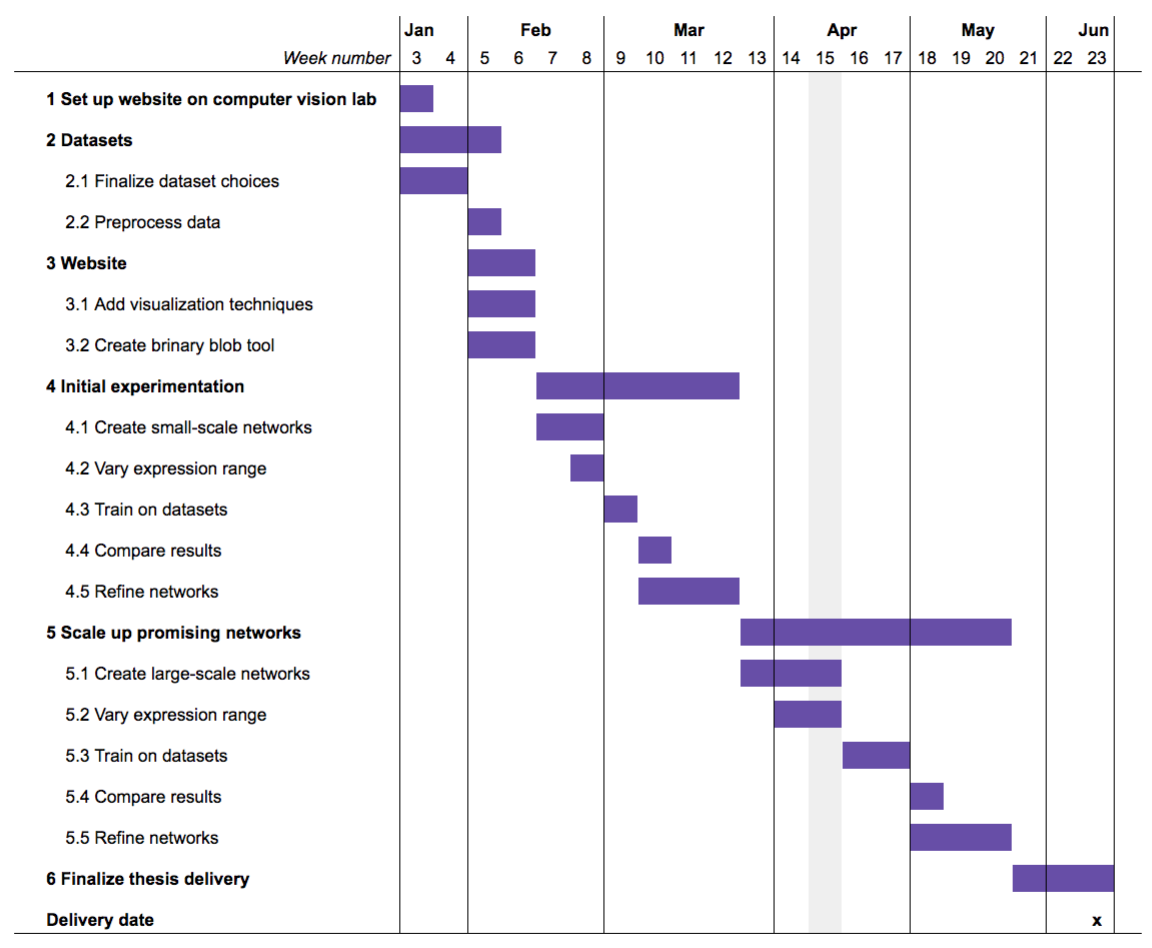
\includegraphics[scale=0.7]{images/gantt_diagram.png}
\end{figure}

% Bibliography - edit references.bib and use the \cite command in text
\bibliographystyle{plain}
\bibliography{references}
\end{document}
